% Created by tikzDevice version 0.12.3 on 2020-01-31 11:14:13
% !TEX encoding = UTF-8 Unicode
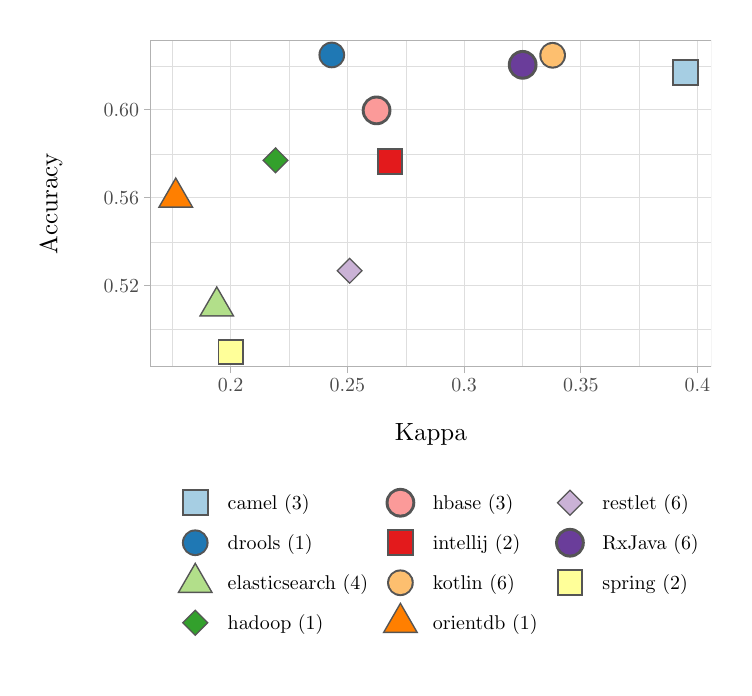
\begin{tikzpicture}[x=1pt,y=1pt]
\definecolor{fillColor}{RGB}{255,255,255}
\path[use as bounding box,fill=fillColor,fill opacity=0.00] (0,0) rectangle (251.50,231.26);
\begin{scope}
\path[clip] (  0.00,  0.00) rectangle (251.50,231.26);
\definecolor{drawColor}{RGB}{255,255,255}
\definecolor{fillColor}{RGB}{255,255,255}

\path[draw=drawColor,line width= 0.5pt,line join=round,line cap=round,fill=fillColor] (  0.00,  0.00) rectangle (251.50,231.26);
\end{scope}
\begin{scope}
\path[clip] ( 44.29,108.67) rectangle (247.00,226.76);
\definecolor{fillColor}{RGB}{255,255,255}

\path[fill=fillColor] ( 44.29,108.67) rectangle (247.00,226.76);
\definecolor{drawColor}{gray}{0.87}

\path[draw=drawColor,line width= 0.1pt,line join=round] ( 44.29,122.15) --
	(247.00,122.15);

\path[draw=drawColor,line width= 0.1pt,line join=round] ( 44.29,153.93) --
	(247.00,153.93);

\path[draw=drawColor,line width= 0.1pt,line join=round] ( 44.29,185.72) --
	(247.00,185.72);

\path[draw=drawColor,line width= 0.1pt,line join=round] ( 44.29,217.51) --
	(247.00,217.51);

\path[draw=drawColor,line width= 0.1pt,line join=round] ( 52.29,108.67) --
	( 52.29,226.76);

\path[draw=drawColor,line width= 0.1pt,line join=round] ( 94.46,108.67) --
	( 94.46,226.76);

\path[draw=drawColor,line width= 0.1pt,line join=round] (136.62,108.67) --
	(136.62,226.76);

\path[draw=drawColor,line width= 0.1pt,line join=round] (178.78,108.67) --
	(178.78,226.76);

\path[draw=drawColor,line width= 0.1pt,line join=round] (220.94,108.67) --
	(220.94,226.76);

\path[draw=drawColor,line width= 0.2pt,line join=round] ( 44.29,138.04) --
	(247.00,138.04);

\path[draw=drawColor,line width= 0.2pt,line join=round] ( 44.29,169.83) --
	(247.00,169.83);

\path[draw=drawColor,line width= 0.2pt,line join=round] ( 44.29,201.61) --
	(247.00,201.61);

\path[draw=drawColor,line width= 0.2pt,line join=round] ( 73.37,108.67) --
	( 73.37,226.76);

\path[draw=drawColor,line width= 0.2pt,line join=round] (115.54,108.67) --
	(115.54,226.76);

\path[draw=drawColor,line width= 0.2pt,line join=round] (157.70,108.67) --
	(157.70,226.76);

\path[draw=drawColor,line width= 0.2pt,line join=round] (199.86,108.67) --
	(199.86,226.76);

\path[draw=drawColor,line width= 0.2pt,line join=round] (242.02,108.67) --
	(242.02,226.76);
\definecolor{fillColor}{RGB}{85,85,85}

\path[fill=fillColor] (111.52,143.42) --
	(116.34,148.23) --
	(121.15,143.42) --
	(116.34,138.60) --
	cycle;

\path[fill=fillColor] (189.69,221.28) circle (  4.82);
\definecolor{drawColor}{RGB}{85,85,85}

\path[draw=drawColor,line width= 1.1pt,line join=round,line cap=round,fill=fillColor] (178.86,217.83) circle (  4.82);

\path[fill=fillColor] ( 68.33,138.06) --
	( 74.81,126.83) --
	( 61.84,126.83) --
	cycle;

\path[fill=fillColor] (232.97,210.24) --
	(242.60,210.24) --
	(242.60,219.87) --
	(232.97,219.87) --
	cycle;

\path[draw=drawColor,line width= 1.1pt,line join=round,line cap=round,fill=fillColor] (126.07,201.37) circle (  4.82);

\path[fill=fillColor] (126.09,178.14) --
	(135.72,178.14) --
	(135.72,187.77) --
	(126.09,187.77) --
	cycle;

\path[fill=fillColor] ( 68.60,109.22) --
	( 78.23,109.22) --
	( 78.23,118.86) --
	( 68.60,118.86) --
	cycle;

\path[fill=fillColor] ( 84.74,183.31) --
	( 89.56,188.13) --
	( 94.37,183.31) --
	( 89.56,178.50) --
	cycle;

\path[fill=fillColor] (109.89,221.40) circle (  4.82);

\path[fill=fillColor] ( 53.51,177.40) --
	( 59.99,166.16) --
	( 47.02,166.16) --
	cycle;
\definecolor{fillColor}{RGB}{202,178,214}

\path[fill=fillColor] (112.23,143.42) --
	(116.34,147.52) --
	(120.44,143.42) --
	(116.34,139.31) --
	cycle;
\definecolor{fillColor}{RGB}{253,191,111}

\path[fill=fillColor] (189.69,221.28) circle (  4.10);
\definecolor{drawColor}{RGB}{106,61,154}
\definecolor{fillColor}{RGB}{106,61,154}

\path[draw=drawColor,line width= 0.4pt,line join=round,line cap=round,fill=fillColor] (178.86,217.83) circle (  4.10);
\definecolor{fillColor}{RGB}{178,223,138}

\path[fill=fillColor] ( 68.33,136.96) --
	( 73.86,127.38) --
	( 62.80,127.38) --
	cycle;
\definecolor{fillColor}{RGB}{166,206,227}

\path[fill=fillColor] (233.68,210.95) --
	(241.89,210.95) --
	(241.89,219.16) --
	(233.68,219.16) --
	cycle;
\definecolor{drawColor}{RGB}{251,154,153}
\definecolor{fillColor}{RGB}{251,154,153}

\path[draw=drawColor,line width= 0.4pt,line join=round,line cap=round,fill=fillColor] (126.07,201.37) circle (  4.10);
\definecolor{fillColor}{RGB}{227,26,28}

\path[fill=fillColor] (126.80,178.85) --
	(135.00,178.85) --
	(135.00,187.05) --
	(126.80,187.05) --
	cycle;
\definecolor{fillColor}{RGB}{255,255,153}

\path[fill=fillColor] ( 69.31,109.94) --
	( 77.52,109.94) --
	( 77.52,118.14) --
	( 69.31,118.14) --
	cycle;
\definecolor{fillColor}{RGB}{51,160,44}

\path[fill=fillColor] ( 85.45,183.31) --
	( 89.56,187.42) --
	( 93.66,183.31) --
	( 89.56,179.21) --
	cycle;
\definecolor{fillColor}{RGB}{31,120,180}

\path[fill=fillColor] (109.89,221.40) circle (  4.10);
\definecolor{fillColor}{RGB}{255,127,0}

\path[fill=fillColor] ( 53.51,176.29) --
	( 59.04,166.72) --
	( 47.98,166.72) --
	cycle;
\definecolor{drawColor}{gray}{0.70}

\path[draw=drawColor,line width= 0.5pt,line join=round,line cap=round] ( 44.29,108.67) rectangle (247.00,226.76);
\end{scope}
\begin{scope}
\path[clip] (  0.00,  0.00) rectangle (251.50,231.26);
\definecolor{drawColor}{gray}{0.30}

\node[text=drawColor,anchor=base east,inner sep=0pt, outer sep=0pt, scale=  0.72] at ( 40.24,135.56) {0.52};

\node[text=drawColor,anchor=base east,inner sep=0pt, outer sep=0pt, scale=  0.72] at ( 40.24,167.35) {0.56};

\node[text=drawColor,anchor=base east,inner sep=0pt, outer sep=0pt, scale=  0.72] at ( 40.24,199.13) {0.60};
\end{scope}
\begin{scope}
\path[clip] (  0.00,  0.00) rectangle (251.50,231.26);
\definecolor{drawColor}{gray}{0.70}

\path[draw=drawColor,line width= 0.2pt,line join=round] ( 42.04,138.04) --
	( 44.29,138.04);

\path[draw=drawColor,line width= 0.2pt,line join=round] ( 42.04,169.83) --
	( 44.29,169.83);

\path[draw=drawColor,line width= 0.2pt,line join=round] ( 42.04,201.61) --
	( 44.29,201.61);
\end{scope}
\begin{scope}
\path[clip] (  0.00,  0.00) rectangle (251.50,231.26);
\definecolor{drawColor}{gray}{0.70}

\path[draw=drawColor,line width= 0.2pt,line join=round] ( 73.37,106.42) --
	( 73.37,108.67);

\path[draw=drawColor,line width= 0.2pt,line join=round] (115.54,106.42) --
	(115.54,108.67);

\path[draw=drawColor,line width= 0.2pt,line join=round] (157.70,106.42) --
	(157.70,108.67);

\path[draw=drawColor,line width= 0.2pt,line join=round] (199.86,106.42) --
	(199.86,108.67);

\path[draw=drawColor,line width= 0.2pt,line join=round] (242.02,106.42) --
	(242.02,108.67);
\end{scope}
\begin{scope}
\path[clip] (  0.00,  0.00) rectangle (251.50,231.26);
\definecolor{drawColor}{gray}{0.30}

\node[text=drawColor,anchor=base,inner sep=0pt, outer sep=0pt, scale=  0.72] at ( 73.37, 99.66) {0.2};

\node[text=drawColor,anchor=base,inner sep=0pt, outer sep=0pt, scale=  0.72] at (115.54, 99.66) {0.25};

\node[text=drawColor,anchor=base,inner sep=0pt, outer sep=0pt, scale=  0.72] at (157.70, 99.66) {0.3};

\node[text=drawColor,anchor=base,inner sep=0pt, outer sep=0pt, scale=  0.72] at (199.86, 99.66) {0.35};

\node[text=drawColor,anchor=base,inner sep=0pt, outer sep=0pt, scale=  0.72] at (242.02, 99.66) {0.4};
\end{scope}
\begin{scope}
\path[clip] (  0.00,  0.00) rectangle (251.50,231.26);
\definecolor{drawColor}{RGB}{0,0,0}

\node[text=drawColor,anchor=base,inner sep=0pt, outer sep=0pt, scale=  0.90] at (145.65, 82.07) {Kappa};
\end{scope}
\begin{scope}
\path[clip] (  0.00,  0.00) rectangle (251.50,231.26);
\definecolor{drawColor}{RGB}{0,0,0}

\node[text=drawColor,rotate= 90.00,anchor=base,inner sep=0pt, outer sep=0pt, scale=  0.90] at ( 10.70,167.72) {Accuracy};
\end{scope}
\begin{scope}
\path[clip] (  0.00,  0.00) rectangle (251.50,231.26);
\definecolor{fillColor}{RGB}{255,255,255}

\path[fill=fillColor] ( 44.32,  4.50) rectangle (246.97, 71.32);
\end{scope}
\begin{scope}
\path[clip] (  0.00,  0.00) rectangle (251.50,231.26);
\definecolor{fillColor}{RGB}{255,255,255}

\path[fill=fillColor] ( 53.32, 52.36) rectangle ( 67.78, 66.82);
\end{scope}
\begin{scope}
\path[clip] (  0.00,  0.00) rectangle (251.50,231.26);
\definecolor{fillColor}{RGB}{85,85,85}

\path[fill=fillColor] ( 55.73, 54.77) --
	( 65.36, 54.77) --
	( 65.36, 64.40) --
	( 55.73, 64.40) --
	cycle;
\end{scope}
\begin{scope}
\path[clip] (  0.00,  0.00) rectangle (251.50,231.26);
\definecolor{fillColor}{RGB}{166,206,227}

\path[fill=fillColor] ( 56.44, 55.48) --
	( 64.65, 55.48) --
	( 64.65, 63.69) --
	( 56.44, 63.69) --
	cycle;
\end{scope}
\begin{scope}
\path[clip] (  0.00,  0.00) rectangle (251.50,231.26);
\definecolor{fillColor}{RGB}{255,255,255}

\path[fill=fillColor] ( 53.32, 37.91) rectangle ( 67.78, 52.36);
\end{scope}
\begin{scope}
\path[clip] (  0.00,  0.00) rectangle (251.50,231.26);
\definecolor{fillColor}{RGB}{85,85,85}

\path[fill=fillColor] ( 60.55, 45.14) circle (  4.82);
\end{scope}
\begin{scope}
\path[clip] (  0.00,  0.00) rectangle (251.50,231.26);
\definecolor{fillColor}{RGB}{31,120,180}

\path[fill=fillColor] ( 60.55, 45.14) circle (  4.10);
\end{scope}
\begin{scope}
\path[clip] (  0.00,  0.00) rectangle (251.50,231.26);
\definecolor{fillColor}{RGB}{255,255,255}

\path[fill=fillColor] ( 53.32, 23.45) rectangle ( 67.78, 37.91);
\end{scope}
\begin{scope}
\path[clip] (  0.00,  0.00) rectangle (251.50,231.26);
\definecolor{fillColor}{RGB}{85,85,85}

\path[fill=fillColor] ( 60.55, 38.17) --
	( 67.03, 26.94) --
	( 54.06, 26.94) --
	cycle;
\end{scope}
\begin{scope}
\path[clip] (  0.00,  0.00) rectangle (251.50,231.26);
\definecolor{fillColor}{RGB}{178,223,138}

\path[fill=fillColor] ( 60.55, 37.06) --
	( 66.08, 27.49) --
	( 55.02, 27.49) --
	cycle;
\end{scope}
\begin{scope}
\path[clip] (  0.00,  0.00) rectangle (251.50,231.26);
\definecolor{fillColor}{RGB}{255,255,255}

\path[fill=fillColor] ( 53.32,  9.00) rectangle ( 67.78, 23.45);
\end{scope}
\begin{scope}
\path[clip] (  0.00,  0.00) rectangle (251.50,231.26);
\definecolor{fillColor}{RGB}{85,85,85}

\path[fill=fillColor] ( 55.73, 16.23) --
	( 60.55, 21.04) --
	( 65.36, 16.23) --
	( 60.55, 11.41) --
	cycle;
\end{scope}
\begin{scope}
\path[clip] (  0.00,  0.00) rectangle (251.50,231.26);
\definecolor{fillColor}{RGB}{51,160,44}

\path[fill=fillColor] ( 56.44, 16.23) --
	( 60.55, 20.33) --
	( 64.65, 16.23) --
	( 60.55, 12.12) --
	cycle;
\end{scope}
\begin{scope}
\path[clip] (  0.00,  0.00) rectangle (251.50,231.26);
\definecolor{fillColor}{RGB}{255,255,255}

\path[fill=fillColor] (127.46, 52.36) rectangle (141.92, 66.82);
\end{scope}
\begin{scope}
\path[clip] (  0.00,  0.00) rectangle (251.50,231.26);
\definecolor{drawColor}{RGB}{85,85,85}
\definecolor{fillColor}{RGB}{85,85,85}

\path[draw=drawColor,line width= 1.1pt,line join=round,line cap=round,fill=fillColor] (134.69, 59.59) circle (  4.82);
\end{scope}
\begin{scope}
\path[clip] (  0.00,  0.00) rectangle (251.50,231.26);
\definecolor{drawColor}{RGB}{251,154,153}
\definecolor{fillColor}{RGB}{251,154,153}

\path[draw=drawColor,line width= 0.4pt,line join=round,line cap=round,fill=fillColor] (134.69, 59.59) circle (  4.10);
\end{scope}
\begin{scope}
\path[clip] (  0.00,  0.00) rectangle (251.50,231.26);
\definecolor{fillColor}{RGB}{255,255,255}

\path[fill=fillColor] (127.46, 37.91) rectangle (141.92, 52.36);
\end{scope}
\begin{scope}
\path[clip] (  0.00,  0.00) rectangle (251.50,231.26);
\definecolor{fillColor}{RGB}{85,85,85}

\path[fill=fillColor] (129.87, 40.32) --
	(139.51, 40.32) --
	(139.51, 49.95) --
	(129.87, 49.95) --
	cycle;
\end{scope}
\begin{scope}
\path[clip] (  0.00,  0.00) rectangle (251.50,231.26);
\definecolor{fillColor}{RGB}{227,26,28}

\path[fill=fillColor] (130.59, 41.03) --
	(138.79, 41.03) --
	(138.79, 49.24) --
	(130.59, 49.24) --
	cycle;
\end{scope}
\begin{scope}
\path[clip] (  0.00,  0.00) rectangle (251.50,231.26);
\definecolor{fillColor}{RGB}{255,255,255}

\path[fill=fillColor] (127.46, 23.45) rectangle (141.92, 37.91);
\end{scope}
\begin{scope}
\path[clip] (  0.00,  0.00) rectangle (251.50,231.26);
\definecolor{fillColor}{RGB}{85,85,85}

\path[fill=fillColor] (134.69, 30.68) circle (  4.82);
\end{scope}
\begin{scope}
\path[clip] (  0.00,  0.00) rectangle (251.50,231.26);
\definecolor{fillColor}{RGB}{253,191,111}

\path[fill=fillColor] (134.69, 30.68) circle (  4.10);
\end{scope}
\begin{scope}
\path[clip] (  0.00,  0.00) rectangle (251.50,231.26);
\definecolor{fillColor}{RGB}{255,255,255}

\path[fill=fillColor] (127.46,  9.00) rectangle (141.92, 23.45);
\end{scope}
\begin{scope}
\path[clip] (  0.00,  0.00) rectangle (251.50,231.26);
\definecolor{fillColor}{RGB}{85,85,85}

\path[fill=fillColor] (134.69, 23.72) --
	(141.18, 12.48) --
	(128.20, 12.48) --
	cycle;
\end{scope}
\begin{scope}
\path[clip] (  0.00,  0.00) rectangle (251.50,231.26);
\definecolor{fillColor}{RGB}{255,127,0}

\path[fill=fillColor] (134.69, 22.61) --
	(140.22, 13.04) --
	(129.16, 13.04) --
	cycle;
\end{scope}
\begin{scope}
\path[clip] (  0.00,  0.00) rectangle (251.50,231.26);
\definecolor{fillColor}{RGB}{255,255,255}

\path[fill=fillColor] (188.73, 52.36) rectangle (203.18, 66.82);
\end{scope}
\begin{scope}
\path[clip] (  0.00,  0.00) rectangle (251.50,231.26);
\definecolor{fillColor}{RGB}{85,85,85}

\path[fill=fillColor] (191.14, 59.59) --
	(195.95, 64.40) --
	(200.77, 59.59) --
	(195.95, 54.77) --
	cycle;
\end{scope}
\begin{scope}
\path[clip] (  0.00,  0.00) rectangle (251.50,231.26);
\definecolor{fillColor}{RGB}{202,178,214}

\path[fill=fillColor] (191.85, 59.59) --
	(195.95, 63.69) --
	(200.06, 59.59) --
	(195.95, 55.48) --
	cycle;
\end{scope}
\begin{scope}
\path[clip] (  0.00,  0.00) rectangle (251.50,231.26);
\definecolor{fillColor}{RGB}{255,255,255}

\path[fill=fillColor] (188.73, 37.91) rectangle (203.18, 52.36);
\end{scope}
\begin{scope}
\path[clip] (  0.00,  0.00) rectangle (251.50,231.26);
\definecolor{drawColor}{RGB}{85,85,85}
\definecolor{fillColor}{RGB}{85,85,85}

\path[draw=drawColor,line width= 1.1pt,line join=round,line cap=round,fill=fillColor] (195.95, 45.14) circle (  4.82);
\end{scope}
\begin{scope}
\path[clip] (  0.00,  0.00) rectangle (251.50,231.26);
\definecolor{drawColor}{RGB}{106,61,154}
\definecolor{fillColor}{RGB}{106,61,154}

\path[draw=drawColor,line width= 0.4pt,line join=round,line cap=round,fill=fillColor] (195.95, 45.14) circle (  4.10);
\end{scope}
\begin{scope}
\path[clip] (  0.00,  0.00) rectangle (251.50,231.26);
\definecolor{fillColor}{RGB}{255,255,255}

\path[fill=fillColor] (188.73, 23.45) rectangle (203.18, 37.91);
\end{scope}
\begin{scope}
\path[clip] (  0.00,  0.00) rectangle (251.50,231.26);
\definecolor{fillColor}{RGB}{85,85,85}

\path[fill=fillColor] (191.14, 25.87) --
	(200.77, 25.87) --
	(200.77, 35.50) --
	(191.14, 35.50) --
	cycle;
\end{scope}
\begin{scope}
\path[clip] (  0.00,  0.00) rectangle (251.50,231.26);
\definecolor{fillColor}{RGB}{255,255,153}

\path[fill=fillColor] (191.85, 26.58) --
	(200.06, 26.58) --
	(200.06, 34.79) --
	(191.85, 34.79) --
	cycle;
\end{scope}
\begin{scope}
\path[clip] (  0.00,  0.00) rectangle (251.50,231.26);
\definecolor{drawColor}{RGB}{0,0,0}

\node[text=drawColor,anchor=base west,inner sep=0pt, outer sep=0pt, scale=  0.72] at ( 72.28, 57.11) {camel (3)};
\end{scope}
\begin{scope}
\path[clip] (  0.00,  0.00) rectangle (251.50,231.26);
\definecolor{drawColor}{RGB}{0,0,0}

\node[text=drawColor,anchor=base west,inner sep=0pt, outer sep=0pt, scale=  0.72] at ( 72.28, 42.66) {drools (1)};
\end{scope}
\begin{scope}
\path[clip] (  0.00,  0.00) rectangle (251.50,231.26);
\definecolor{drawColor}{RGB}{0,0,0}

\node[text=drawColor,anchor=base west,inner sep=0pt, outer sep=0pt, scale=  0.72] at ( 72.28, 28.20) {elasticsearch (4)};
\end{scope}
\begin{scope}
\path[clip] (  0.00,  0.00) rectangle (251.50,231.26);
\definecolor{drawColor}{RGB}{0,0,0}

\node[text=drawColor,anchor=base west,inner sep=0pt, outer sep=0pt, scale=  0.72] at ( 72.28, 13.75) {hadoop (1)};
\end{scope}
\begin{scope}
\path[clip] (  0.00,  0.00) rectangle (251.50,231.26);
\definecolor{drawColor}{RGB}{0,0,0}

\node[text=drawColor,anchor=base west,inner sep=0pt, outer sep=0pt, scale=  0.72] at (146.42, 57.11) {hbase (3)};
\end{scope}
\begin{scope}
\path[clip] (  0.00,  0.00) rectangle (251.50,231.26);
\definecolor{drawColor}{RGB}{0,0,0}

\node[text=drawColor,anchor=base west,inner sep=0pt, outer sep=0pt, scale=  0.72] at (146.42, 42.66) {intellij (2)};
\end{scope}
\begin{scope}
\path[clip] (  0.00,  0.00) rectangle (251.50,231.26);
\definecolor{drawColor}{RGB}{0,0,0}

\node[text=drawColor,anchor=base west,inner sep=0pt, outer sep=0pt, scale=  0.72] at (146.42, 28.20) {kotlin (6)};
\end{scope}
\begin{scope}
\path[clip] (  0.00,  0.00) rectangle (251.50,231.26);
\definecolor{drawColor}{RGB}{0,0,0}

\node[text=drawColor,anchor=base west,inner sep=0pt, outer sep=0pt, scale=  0.72] at (146.42, 13.75) {orientdb (1)};
\end{scope}
\begin{scope}
\path[clip] (  0.00,  0.00) rectangle (251.50,231.26);
\definecolor{drawColor}{RGB}{0,0,0}

\node[text=drawColor,anchor=base west,inner sep=0pt, outer sep=0pt, scale=  0.72] at (207.68, 57.11) {restlet (6)};
\end{scope}
\begin{scope}
\path[clip] (  0.00,  0.00) rectangle (251.50,231.26);
\definecolor{drawColor}{RGB}{0,0,0}

\node[text=drawColor,anchor=base west,inner sep=0pt, outer sep=0pt, scale=  0.72] at (207.68, 42.66) {RxJava (6)};
\end{scope}
\begin{scope}
\path[clip] (  0.00,  0.00) rectangle (251.50,231.26);
\definecolor{drawColor}{RGB}{0,0,0}

\node[text=drawColor,anchor=base west,inner sep=0pt, outer sep=0pt, scale=  0.72] at (207.68, 28.20) {spring (2)};
\end{scope}
\end{tikzpicture}
